\chapter{Compilers and analysis tools}\label{chap:tools}

In the~previous chapter, the~reader was introduced to a~branch of~program
ana\-ly\-sis. 
The techniques discussed above focused on both the~static and runtime
side of~program analysis. 

Regardless of~whether these approaches have been implemented, it was 
required to find a~suitable tool for source code manipulation for two reasons. 
First, any external tool output might require altering the~input source code 
based on its output. 
Second, if implementing any code reducing algorithm would have to occur, 
one would need a~sophisticated code modifying framework. 

Due to these reasons, an analysis of~compilers and tools for C and C++ was conducted. 
The goal of~the~analysis is to pick the~most practical tool available. 
Required criteria include frequent upkeep of~the~framework, 
an existing user base, and the~ability to manipulate some abstract 
representation of~the~code.

The representation boiled down to an abstract syntax tree (AST). 
AST embodies the~syntactic structure of~the~code, regardless of~the~code's language. 
A vertex of~an AST represents a~construct of~the~code while not being concrete 
with the~details of the code's programming language. 
This generality is perfect for C and C++'s chosen domain, 
as both languages only differ syntax-wise in~minor details.

Below are the~findings concerning the~most important candidates.

\section{GCC}

A well-known C and C++ compiler, the~GNU Compiler Collection \citep{gcc:online} 
is an extensive
open source project. 
As popular as GCC is, it does not provide the~features an analysis-tool-building 
developer needs. 

For the~sake of~building such tools, a~compiler front end is used. 
Due to an old design, it is difficult to work with either the~front end or 
the back end of~GCC alone. 
Besides, the~compiler implicitly makes optimizations that destroy any parallels 
between the~source code and the~AST. 
Therefore, the~AST has to be treated as an entirely different object rather than 
an abstraction of~the~code. 
Most of~the~compiler's source code representation is unintuitive and 
hard to pick up for anyone not actively contributing to GCC. 
Figure~\ref{img:gcc} showcases the~unfriendliness rather well.
Compared to Figure~\ref{img:pdg}, which is an output of~a~tool built using
LLVM and Clang, GCC's mapping between the~source code and the~internal
representation does not hold up.

As far as AST manipulation is concerned, the~compiler allows the~user to dump 
the structure into a~text representation. 
However, due to the~difficulties mentioned above, it can hardly be used.

\begin{figure}[p]\centering
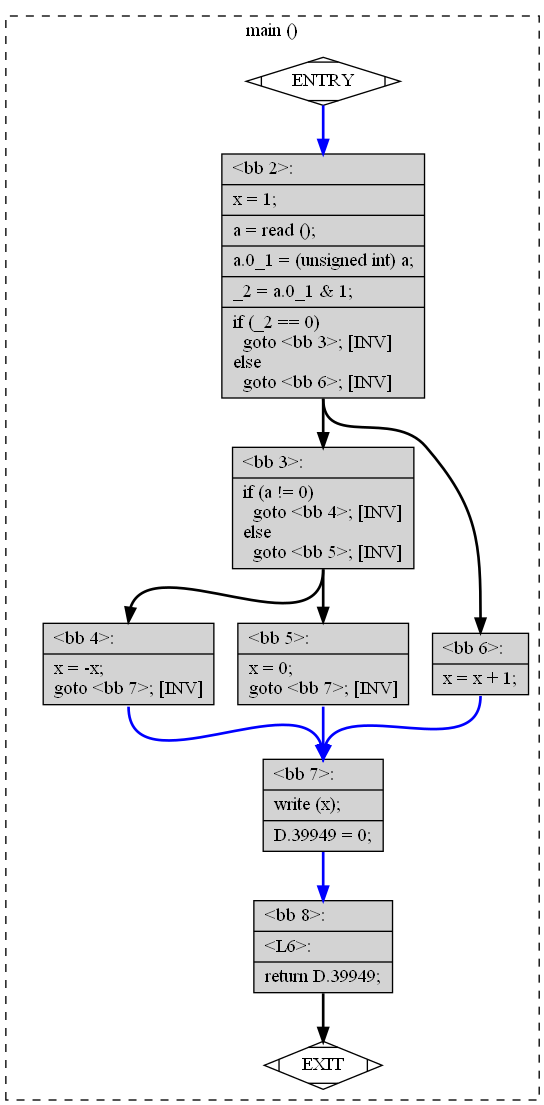
\includegraphics[scale=0.55]{gcc_ast}
\caption{GCC AST Dump. This figure showcases 
the AST representation of Listing~\ref{lst:simpleexample}
as dumped by GCC. Note that it is not easily comprehendable.}
\label{img:gcc}
\end{figure}

These issues result in~a seldom-used variant that offers nearly 
no developer-friendly features. 
An upside is that GCC allows the~user to visualize the~AST. 
However, that is hardly a~useful feature in~the context of~this project.

\section{Clang}

Thanks to LLVM \citep{llvm:online}, the~widespread compiler infrastructure,
the Clang project \citep{clang:online}
has provided a~compiler front end not only for C and C++ but also 
for CUDA, OpenCL, and other mainstream programming languages. 
The extend of~Clang as a~compiler front end is so vast that it covers 
both the~C++ standard and the~unofficial GNU++ dialect.

The project does not include just the~front end but also a~static analyzer 
and several code analysis tools, which are now commonly used in~IDE's as 
syntax and semantic checks. 

This description of~Clang foreshadows its friendliness to analysis tool developers. 
The fact that the~front end runs on a~common intermediate language also indicates 
that openly working with abstract code representations is supported.

There are three most notable interfaces for customizing Clang. 
Firstly, the LibClang interface allows the~users to write 
comprehend-able high-level code with limited functionality. 
On the~other hand, LibTooling gives the~user much more control 
at the~cost of~a~steep learning curve. 
Lastly, the~Plugins interface features similar difficulty 
as LibTooling with a~more specific goal. 
Plugins are used with the~Clang compiler and can be run 
as a~front-end action when called during compilation.

\section{ANTLR}

A less typical way of~extracting an AST from a~source file is by using grammar
recognition.
ANTLR \citep{antlr:online}, which stands for Another Tool for 
Language Recognition, is a~free 
parser generator that generates both a~lexer and a~parser based on 
a given grammar.
Additionally, ANTLR can also generate a~tree parser.
Tree parsers are helpful in~processing ASTs.

The tool is generally used to read data formats, process expressions 
of various query languages, and even parse source code written in complex 
programming languages.
It can be used to generate a~syntax tree and walk through it using a~visitor.
ANTLR is based on the~LL parser, which parses the~input from left to right, 
performing its leftmost derivation.

To create a~parser or a~syntax tree of~code written in a~programming language, 
ANTLR requires the complete grammar of~that language.
Some programming languages, namely C and C++, have an ambiguous syntax that 
is hard to parse based solely on its grammar.
Due to ANTLR's high popularity, many grammars have already been written 
for it.
As far as C++ is concerned, its C++14 standard's grammar is the~most recent 
one available.

Writing grammar for newer standards or creating a~custom one for both C and 
C++ would be unnecessarily burdensome for this project.
This statement holds, especially when considering other tools mentioned above.

The most recent release, ANTLR 4, added more options for grammar rules.
Most notably, it supports direct left recursion.
However, that still might not be enough to choose it over other tools.


\section{DMS}

Similar to ANTLR, the~DMS Software Reengineering Toolkit \citep{dms:online}
features a~parser generator.
The tool is proprietary software created by Semantic Designs.
Besides the~mentioned parser generator, it features an entire toolkit for 
creating custom software analysis.
This toolkit is used mainly for reliable refactoring, duplicate code 
detection, and migration of the source code's programming language.

The parser generator part takes a~grammar and produces a~parser.
This parser then constructs abstract syntax trees for provided source code.
Additionally, created ASTs can be converted back to source code using 
prettyprinters.
The parser saves additional information about provided source files, such as 
comments and formatting.
It can then recreate the~file accurately.

DMS provides a~grammar for a~large number of~programming languages, 
including C and C++.
The language support, however, is not always up-to-date.
The newest supported C++ standard is still the~older C++17.
These complicated grammars' ambiguity is avoided using a~generalized 
left-to-right parser, which performs the~rightmost derivation (GLR).
Since DMS provides refactoring ability as well, it allows for transformation 
rules in~the grammar.

Another helpful feature of~the~toolkit is control flow and data flow analysis.
Analyzing control flow and data flow, generating their graphs, and performing 
the points-to analysis (also supported by DMS) is practical when considering
static slicing (section 1.2).

It should be noted that some of~the~free, open-source tools mentioned above 
do a~better job of~being a~so-called 'software analysis toolkit' than 
DMS does.

\section{Summary}

The chapter highlighted a~spectrum of~tools, ranging from language
recognizers to compilers.

It would seem that parsing source code written in multiple programming 
languages into an abstract representation requires a~common intermediate 
language, in~which the representation is stored. 
Having an intermediate language is not always possible for several reasons, 
including licensing and old architecture. 
The compiler giant GCC seems to suffer from precisely that.
Additionally, since the~Clang project is being contributed to regularly, 
resulting in~as many as five releases per year, 
it pulls in~a more significant developer community. 

Therefore, Clang is the~favorite source code altering tool for this project. 
In the~following chapter, the~relevant parts of~the~Clang project 
will be broken down and explained.
